\RequirePackage{fix-cm}
\documentclass[smallextended,natbib]{svjour3}
\usepackage[T1]{fontenc}
\usepackage[utf8]{inputenc}
\usepackage{url}
\usepackage[colorlinks,linkcolor=blue,citecolor=blue,urlcolor=blue]{hyperref}
\usepackage[autolanguage]{numprint}
\usepackage{booktabs}
\usepackage{graphicx}
\usepackage{wasysym}
\usepackage{fancyvrb}
\usepackage{fvextra}
\usepackage{setspace}
\usepackage{tikz}
\usepackage{cprotect}
\usepackage{float}
\usepackage{adjustbox}
\usepackage{enumitem}

\usepackage{xspace}
\newcommand*{\TODO}{\textcolor{red}{TODO}\xspace}

\newcommand{\num}[1]{\numprint{#1}}
\newcommand{\per}[1]{\numprint[\%]{#1}}

\newenvironment{CVerbatim}
  {\center\BVerbatim}
  {\endBVerbatim\endcenter}

\newcommand{\alias}[2]{{\texttt{#1} $\rightarrow$ \texttt{#2}}}
\newcommand{\cmd}[1]{{\texttt{#1}}}

\journalname{Empirical Software Engineering}

\begin{document}

\title{An Empirical Investigation of Command-Line Customization}

\author{Michael Schröder \and Jürgen Cito}
\institute{%
	Michael Schröder
	\at TU Wien, Vienna, Austria\\
	\email{michael.schroeder@tuwien.ac.at}
	\and
	Jürgen Cito
	\at TU Wien \& MIT, Cambridge, MA\\
	\email{jcito@mit.edu}
}

\maketitle

\begin{abstract}
	The interactive command line, also known as the shell, is a prominent mechanism used extensively by a wide range of software professionals (engineers, system administrators, data scientists, etc.). Shell customizations can therefore provide insight into the tasks they repeatedly perform, how well the standard environment supports those tasks, and ways in which the environment could be productively extended or modified.
To characterize the patterns and complexities of command-line customization, we mined the collective knowledge of command-line users by analysing more than 2.2 million shell alias definitions found on GitHub.
Shell aliases allow command-line users to customize their environment by defining arbitrarily complex command substitutions.
Using inductive coding methods, we found three types of aliases that each enable a number of customization practices: 
\textsc{Shortcuts} (for \emph{nicknaming commands}, \emph{abbreviating subcommands}, and \emph{bookmarking locations}),
\textsc{Modifications} (for \emph{substituting commands}, \emph{overriding defaults}, \emph{colorizing output}, and \emph{elevating privilege}),
and \textsc{Scripts} (for \emph{transforming data} and \emph{chaining subcommands}).
We conjecture that identifying common customization practices can point to particular usability issues within command-line programs, and that a deeper understanding of these practices can support researchers and tool developers in designing better user experiences.
In addition to our analysis, we provide an extensive reproducibility package in the form of a curated dataset together with well-documented computational notebooks enabling further knowledge discovery and a basis for learning approaches to improve command-line workflows.
	\keywords{Command Line \and Customization Practices \and Collective Knowledge \and Inductive Coding}
\end{abstract}

\section{Introduction}

A command line interface, also called a \emph{shell}, is a textual interface that allows users to interact with the underlying operating system by issuing commands.
Expert users, such as system administrators, software developers, researchers, and data scientists, routinely use the shell as it affords them flexibility and the ability to compose multiple commands.
They perform a variety of tasks on their systems including navigating and interacting with the filesystem (e.g., \verb|ls, mv, cd|), using version control (e.g., \verb|git, hg|), installing packages (e.g., \verb|apt-get, npm|), or dealing with infastructure (e.g., \verb|docker|).
Experts can adapt and play with a multitude of commands and arguments, chaining them together to create more complex workflows.
All this versatility introduces a common problem in user interfaces of recognition over recall~\cite{nielsen:05}, where users have to recall the particularities of syntax and argument combinations, instead of enabling them to use a more recognizable symbol (as in graphical user interfaces).

A way for these experts to introduce recognizability and customize their command line experience is to attach a distinct name to potentially convoluted, but frequently used, command and argument structures.
This can be achieved by defining shell aliases.
An alias substitutes a given name, the \emph{alias}, with a string value that defines an arbitrarily complex command (or chain of commands).
The set of aliases users define provides a window into their preferences expressed as part of their personal configuration.
Many users have publicly shared these configurations on social coding platforms such as GitHub.
To study these preferences, we perform an exploratory analysis of over 4.7 million alias definitions on GitHub, which provides a rich dataset to investigate how command line users customize their tasks and workflows.

We find that aliases have multiple complex use cases:
Users often redefine existing commands to include \emph{default arguments} they want to have implicitly included in every execution, rather than specifying them explicitly.
For instance, aliases for \verb|rm|, \verb|cp|, and \verb|mv| are often redefined to introduce the option \verb|-i| to add the interactive safety feature by default.
Aliases are also introduced to redefine different kinds of misspellings to provide a hand-crafted autocorrect feature in the command line. 
Short, memorable names are often introduced as aliases to simplify complex expressions (the average length of an alias name is 4.43 characters, whereas the average length of its substitution is 21.15).
Aliases were also used as bookmarks to local and remote locations (e.g., \verb|cd| or \verb|ssh| together with complicated paths, URLs, or IP addresses).
When further analyzing the compression induced by aliases, we saw that they are not only used to abbreviate and simplify longer commands and chains.
They were also defined to lend more descriptive names to otherwise cryptic and complicated command and argument structures.
When composition is used in aliases, the structures are most often chained by pipes (\verb|||), where further analysis allowed us to ascertain common data flows between different commands.

Our insights can help improve the usability for particular tools and the command line experience in general.
Our results on default arguments indicate usability issues for a wide range of tools, but also shows that defaults can sometimes be contextual (e.g., \verb|-i| interactive mode by default in the command line, but not when executing scripts).
We also envision that our results and dataset can be used to learn repair rules, in order to correct not only user errors, but also provide usage hints to introduce newcomers to common workflows.

In the following, we introduce more background by describing usage and syntax of aliases. We further describe our data collection and parsing process. We then present results from our exploratory analysis on shell aliases in the wild, following by a discussion on implications for usability. We finally discuss threats to validity and review related work in the broader context of this study. 

\section{Background}

A shell is a command interpreter allowing the user to interact with an underlying system.
The concept of the operating system shell as an independent process executing outside the kernel originated in Multics and was further developed into the original Unix shell \verb|sh| and its various descendants.
%  (\TODO references)
The POSIX family of standards defines a Shell Command Language~\cite{posix_standard, greenberg:17}, whose standard implementation is still the \verb|sh| utility, but there exist a wide variety of popular POSIX-compliant shells like \verb|bash| or \verb|zsh|.
These implementations are free to extend the functionality of the shell, but all share a common subset of core commands and programming language constructs.
In this paper, we focus on the built-in \verb|alias| command, available on all POSIX shells.

\subsection{Usage and Syntax}

The \verb|alias| command allows the user to create \emph{alias definitions}, defining command substitutions.
When the shell processes the command line, it replaces known alias names with their defined string values.
For example, 
\begin{CVerbatim}
alias ll='ls -l'
\end{CVerbatim}
defines the \emph{alias name} \verb|ll|, that is replaced by the \emph{alias value} \verb|ls -l|.
In this case, \verb|ls| is the standard command for listing directory contents, with the argument \verb|-l| specifying a long-form output format.
So the alias \verb|ll| (present in many system configurations) is used to specify a default argument to a commonly used command under a different name.

Alias values can be arbitrarily complex strings and can substitute not only simple commands and arguments, but whole chains of commands. 
The definition
\begin{CVerbatim}
alias ducks="du -cksh * | sort -hr | head -n 15"
\end{CVerbatim}
defines the new command \verb|ducks| by chaining together three different command line tools in order to return the 15 largest files in the current directory.

%alias ip=ifconfig | grep "inet " | grep -v 127.0.0.1 | cut -d' ' -f2
%which chains together several commands to find out the IP addresses of the system.

%alias unwip="git log -n 1 | grep -q -c wip && git reset HEAD~1"
%which chains together three commands to rewind the most recent commit in a git repository, if its commit message contains the word "wip".

In general, an alias definition takes the form
\begin{CVerbatim}
alias name=value
\end{CVerbatim}
where \verb|value| can optionally be enclosed in single (\verb|'|) or double (\verb|"|) quotes and \verb|name| can be any identifier that is a valid command name.\footnote{Some shells allow for an alternative alias syntax without the equals sign between \texttt{name} and \texttt{value}. In this paper we only look at POSIX-compliant alias definitions.}
% TODO: technically not quite correct, see FSE review 2
In particular, the alias name can be an existing command, so a re-definition like
\begin{CVerbatim}
alias grep='grep --color=always'
\end{CVerbatim}
is possible.

\subsection{Dotfiles}

Aliases can be entered directly on the command line, in which case they are valid until the shell session ends.
To make an alias definition permanent, it is common practice to enter it into a file that is read and executed by the shell on startup.
The names of these configuration files differ by shell, but common ones are \verb|.bashrc|, \verb|.zshrc| or \verb|.profile|.
Often, aliases are also stored in other files referred to by these startup scripts.

These kinds of files --- text-based configuration files that store system or application settings --- are also known as \emph{dotfiles}, because their filenames usually start with a dot (\verb|.|) so that they are hidden by default on most Unix-based systems.
In recent years, people have started sharing their dotfiles on platforms like GitHub.\footnote{\url{https://dotfiles.github.io}}
This has the advantage of being able to sync one's configurations across different machines, and also enables exchange and discovery of configurations between users.


\section{Dataset}

Our analysis is based on \num{2204199} alias definitions found on GitHub, collected over a period of two-and-a-half weeks from December 20th 2019 to January 8th 2020.

\subsection{Data Collection}

\begin{figure*}
	\centering
	%\vspace{2em}
	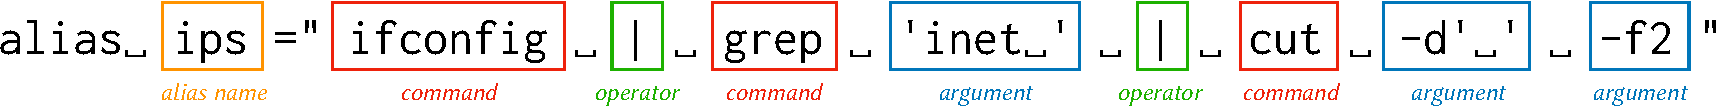
\includegraphics[width=0.85\textwidth]{parser_breakdown.pdf}
	\caption{Decomposition of \texttt{alias ips="ifconfig | grep 'inet ' | cut -d' ' -f2"}.}
	\label{fig:parser}
\end{figure*}

Alias definitions can appear in any Shell script, but we anticipated that they would predominantly be found in personal configuration files (like \verb|.bashrc| or \verb|.bash_profile|).
While we did not want to focus exclusively on these personal configuration scripts, as we want to study the wide range of different alias uses, it is important that they are appropriately accounted for in order for our data to be representative.
Unfortunately, this rules out using some prominent existing datasets for our study~\cite{mombach}:
The public GitHub archive on BigQuery,\footnote{\url{https://bigquery.cloud.google.com/table/bigquery-public-data:github_repos.files}} while containing over 1.5 TB of source code, only includes ``notable projects'' (presumably those with a certain number of stars on GitHub) that additionally have an explicit open source license. 
This leaves out many of the repositories we are interested in, as users sharing configuration scripts for personal use do not usually add a license file and their repositories are generally not ``notable''.
GHTorrent~\cite{ghtorrent}, another popular archive of GitHub data, only contains metadata but not file contents.

Therefore, we found it necessary to write our own tooling to directly collect the data from GitHub ourselves.
We used the GitHub Code Search API to find files written in Shell language\footnote{GitHub uses the Linguist library to classify code: \url{https://github.com/github/linguist}} that contain the string \verb|alias|.

Alas, the GitHub Code Search API comes with its own set of limitations:
\begin{enumerate}
    \item only files smaller than 384 KB are searchable
    \item forks are not included
    \item requests are rate limited at 30 per minute and there are additional opaque abuse detection mechanisms that impose further restrictions in an unforeseeable manner
    \item the number of results is limited to 1000 per search request
\end{enumerate}
The first two limitations do not really affect us, as we are interested in smaller files and do not have to consider forks.
The rate limiting, while significantly slowing down the retrieval process, is also not a fatal obstacle.
The maximum number of returned search results, however, is a critical limitation.
To get around it, we wrote a Python tool called \verb|BLINDED-SEARCHER| that uses a clever sampling strategy to vastly increase the number of results we are able to retrieve.
% \verb|github-searcher|\footnote{\TODO: url/paper} 

The sampling strategy is based on the GitHub API allowing code search queries to be conditioned on file sizes. 
For example, the query 
\begin{CVerbatim}
alias language:Shell size:101..200
\end{CVerbatim}
returns up to 1000 Shell language files containing the string ``alias'' that have a file size between 101 and 200 bytes (inclusive).
Repeating the search with 
\begin{CVerbatim}
alias language:Shell size:201..300
\end{CVerbatim}
returns up to 1000 files of a size between 201 and 300 bytes, and so on.
Repeatedly searching with the same search term but different non-overlapping file size ranges allows us to significantly increase our sample of the overall population.
Another trick further improves on this: 
the API gives us an option to sort the results by most or least recently indexed;
if we run a search using a specific sort order, then we can effectively double the sample size by repeating the same search with the opposite sort order.
Thus we can get up to 2000 results per search per file size range.

Additionally, while GitHub does not allow us to retrieve more than a limited number of files per query, it does return the total count of files matching the query.
While this count is usually very erratic on broad searches, fluctuating wildly between repeated requests, it turns out to be fairly accurate for searches with a small number of results, such as those conditioned on a narrow range of file sizes.
This allows us to get a good estimate of the population, and how accurately our sample approximates it.

For this study, using the search term
\begin{CVerbatim}
alias language:Shell
\end{CVerbatim}
and the sampling strategy described above, we started by sampling all files in increments of 100 bytes and stopped when we reached 29 KB.
We then re-sampled some high-population areas with smaller size increments in order to get a better sample, in some cases sampling in increments of 1 byte.
In total, we collected \num{844140} files from \num{304361} GitHub repositories.
Our sample represents \per{94.09} of the estimated population of \num{897182} files under 29 KB on GitHub written in Shell language and containing the word ``alias''.
The file contents, together with repository metadata, were stored in an SQLite database.
After removing duplicates, our database contains \num{372816} unique files from \num{205126} repositories.

\subsection{Parsing}

After collecting files with potential aliases, we ran a parsing script to find actual alias definitions and decompose them into their constituent parts for analysis.
The decomposed aliases are stored in the same SQLite database as the raw file contents to facilitate easy cross-referencing.
The database schema is given in \Cref{fig:schema}.

\begin{figure}
    \centering
    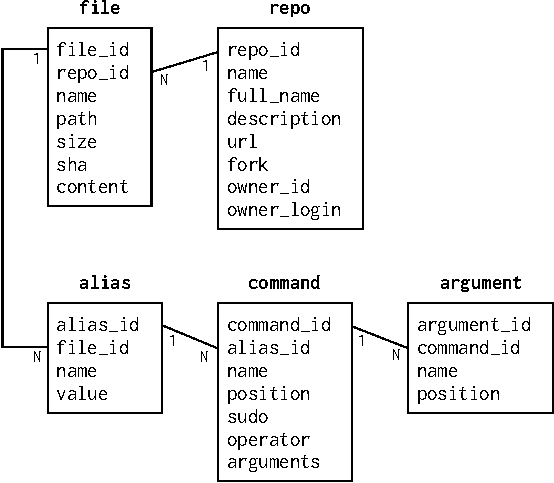
\includegraphics[width=0.9\columnwidth]{schema.pdf}
    \caption{Relational database schema.}
    \label{fig:schema}
\end{figure}

The parser is a Haskell script that splits each alias definition into alias name and alias value, and tokenizes the value into commands and arguments.
Commands can be delimited by the shell operators for piping (\verb!|! and \verb!|&!), logical composition (\verb|&&| and \verb!||!), background execution (\verb|&|) and simple chaining (\verb|;|).
Arguments are separated by whitespace, but care is taken to handle quoted arguments correctly. 
For example, 
\begin{CVerbatim}
echo "hello world"
\end{CVerbatim}
is parsed as one command (\texttt{echo}) with one argument (\texttt{"hello world"}).
See \Cref{fig:parser} for a more elaborate example.

\begin{table*}[t]
    \caption{Top alias names, commands and arguments}
    \label{tab:top-summary}
    \begin{tabular}{lrr}
        \toprule
                 Alias Name &            \# &          \% \\
        \midrule
                  \verb|ls| &  \num{124515} &  \num{2.61} \\
                  \verb|ll| &   \num{89254} &  \num{1.87} \\
         \verb|'${1+"$@"}'| &   \num{78265} &  \num{1.64} \\
                \verb|grep| &   \num{63392} &  \num{1.33} \\
                  \verb|la| &   \num{62039} &  \num{1.30} \\
        \bottomrule
    \end{tabular}
    \hspace{0.3cm}
    \begin{tabular}{lrr}
        \toprule
               Command &            \# &           \% \\
        \midrule
            \verb|git| &  \num{626185} &  \num{11.79} \\
             \verb|ls| &  \num{378097} &   \num{7.12} \\
             \verb|cd| &  \num{229522} &   \num{4.32} \\
           \verb|grep| &  \num{128045} &   \num{2.41} \\
           \verb|"$@"| &   \num{78276} &   \num{1.47} \\
        \bottomrule
    \end{tabular}
    \hspace{0.3cm}
    \begin{tabular}{lrr}
        \toprule
                    Argument &            \# &          \% \\
        \midrule
         \verb|--color=auto| &  \num{268171} &  \num{3.60} \\
                   \verb|-i| &  \num{109094} &  \num{1.47} \\
                   \verb|-v| &   \num{70424} &  \num{0.95} \\
                   \verb|-l| &   \num{63302} &  \num{0.85} \\
                   \verb|-a| &   \num{62023} &  \num{0.83} \\
        \bottomrule
    \end{tabular}        
\end{table*}

Beyond quoting, which is defined by the Shell Command Language and thus uniform across all commands, the parser can not make any further considerations as to how arguments are meant to be interpreted.
While there are some conventions around command line argument handling, programs are generally free to do as they wish and there is a wide variety of argument styles in the wild:
\begin{itemize}
    \item single-dash short arguments combined with double-dash long-form arguments, e.g. \verb|ls -l -a --color=always|
    \item combined short arguments without a dash, e.g. \\ \verb|tar xvzf archive.tar|
    \item dictionary-style arguments, e.g. \\ \verb|dd if=/dev/zero of=/dev/sda|
    \item subcommands, e.g. \verb|git commit -m "wip"|
\end{itemize}
and many more.
Since the parser can not know the intentions of any command, it simply treats each token as a separate argument.
There is one exception: if the command is \texttt{sudo}, then its first argument is taken as the real command. 
For example,
\begin{CVerbatim}
sudo apt-get install
\end{CVerbatim} 
is parsed as the command \texttt{apt-get} with argument \texttt{install} and the sudo flag set.

After parsing, we ended up with \num{2204199} alias definitions, broken down into \num{2534167} commands and \num{3630423} arguments.
Files that did not contain any aliases were removed from the database, as was repository metadata that only referenced files without aliases.
\num{194218} files from \num{138112} repositories, or \per{52.09} of the original sample without duplicates, contained aliases.
The majority of aliases in our dataset (\per{86.2}) originate from common startup scripts, like \texttt{.bashrc} or \texttt{.profile} (see \Cref{tab:file-names}).

\begin{table}
	\caption{Distribution of common file names}
    \label{tab:file-names}
    \begin{tabular}{rrlll}
        \toprule
                  \% &         Files &           Name Pattern &        Aliases &           \% \\
        \midrule
         \num{14.55} &  \num{28255}  &         \verb|*alias*| &  \num{626071}  &   \num{28.4} \\
         \num{27.73} &  \num{53855}  &        \verb|*bashrc*| &  \num{591482}  &  \num{26.83} \\
         \num{22.15} &  \num{43011}  &         \verb|*zshrc*| &  \num{487002}  &  \num{22.09} \\
          \num{9.42} &  \num{18305}  &       \verb|*profile*| &  \num{199168}  &   \num{9.04} \\
        \bottomrule
        \end{tabular}
\end{table}

\subsection{Reproducibility}
\label{sec:reproducibility}

To enable reproducibility and follow-up studies, we have made all data and our entire tool-chain publicly available.
This includes executable Jupyter notebooks used during our analysis, containing all SQL queries and Python code.
Our entire dataset (1.25 GB of parsed alias definitions, plus 4.3 GB unparsed file contents and repository metadata), the parsing script, the notebooks, as well as this paper, are available on GitHub.\footnote{Omitted for double blind review}
%\footnote{\url{https://github.com/ipa-lab/shell-alias-analysis}}


\section{Findings}

\begin{table}
    \caption{Top two commands with top arguments and aliases}
    \label{tab:command-summary}
    \newcommand{\numx}[1]{{\small (\num{#1})}}
\begin{table}
    \caption{Top two commands with top arguments and aliases}
    \label{tab:command-summary}
    \begin{tabular}{@{}lrll@{}}
        \toprule
                    &           \% &            Arguments &                                                                 Aliases (\%) \\
        \midrule
         \verb|git| &   \num{5.85} &        \verb|status| &                              \verb|gs| \numx{54.27}, \verb|gst| \numx{19.19} \\
                    &   \num{3.48} &              \verb|| &                                \verb|g| \numx{75.71}, \verb|gti| \numx{5.74} \\
                    &   \num{3.20} &      \verb|checkout| &      \verb|gco| \numx{50.52}, \verb|gc| \numx{13.87}, \verb|gch| \numx{7.56} \\
                    &   \num{3.18} &          \verb|push| &      \verb|gp| \numx{46.73}, \verb|gps| \numx{9.23}, \verb|push| \numx{7.56} \\
                    &   \num{3.16} &          \verb|diff| &                                                       \verb|gd| \numx{79.89} \\
                    &   \num{2.86} &          \verb|pull| &      \verb|gpl| \numx{18.30}, \verb|gl| \numx{16.59}, \verb|gp| \numx{15.07} \\
                    &   \num{2.78} &        \verb|branch| &                               \verb|gb| \numx{73.54}, \verb|gbr| \numx{6.57} \\
                    &   \num{2.71} &           \verb|add| &                                                       \verb|ga| \numx{80.96} \\
                    &   \num{2.00} &        \verb|commit| &                               \verb|gc| \numx{63.16}, \verb|gci| \numx{5.33} \\
                    &   \num{1.96} &     \verb|commit -m| &       \verb|gcm| \numx{31.29}, \verb|gc| \numx{25.18}, \verb|gm| \numx{7.97} \\
        \midrule
          \verb|ls| &  \num{14.45} &  \verb|--color=auto| &                                                       \verb|ls| \numx{99.04} \\
                    &   \num{8.63} &            \verb|-A| &                                                       \verb|la| \numx{97.61} \\
                    &   \num{7.80} &           \verb|-CF| &                                                        \verb|l| \numx{98.75} \\
                    &   \num{6.78} &          \verb|-alF| &                                                       \verb|ll| \numx{97.49} \\
                    &   \num{5.46} &            \verb|-l| &                                 \verb|ll| \numx{78.83}, \verb|l| \numx{7.91} \\
                    &   \num{3.75} &              \verb|| &                                \verb|l| \numx{27.90}, \verb|sl| \numx{21.45} \\
                    &   \num{2.88} &            \verb|-G| &                                                       \verb|ls| \numx{96.47} \\
                    &   \num{2.74} &           \verb|-la| &      \verb|ll| \numx{38.42}, \verb|la| \numx{26.87}, \verb|lla| \numx{12.63} \\
                    &   \num{2.67} &            \verb|-a| &                                                       \verb|la| \numx{76.94} \\
                    &   \num{1.92} &           \verb|-al| &         \verb|ll| \numx{49.69}, \verb|la| \numx{12.23}, \verb|l| \numx{8.49} \\
        \bottomrule
    \end{tabular}
\end{table}


\end{table}

\Cref{tab:top-summary} shows the most common alias names, commands, and arguments appearing in alias definitions.
The most common alias name we found is \texttt{ls}, appearing a total number of \num{83782} times, which is \per{3.8} of all alias definitions.
Note that this is \texttt{ls} as an \emph{alias name}, a redefinition of the \texttt{ls} \emph{command}, which appears \num{260156} times (\per{10.27}).
This is a bit less often than \texttt{git}, the most common command, which appears in \num{327786} aliases (\per{12.93}).
The most common argument, across all commands, is \texttt{--color=auto}, appearing \num{153931} times (\per{4.24})

Looking at each part of an alias definition in isolation can only get us so far, as arguments only gain meaning in conjunction with commands and alias names can be identical between users, referring to the same command/argument combination, or indeed can overlap, meaning the same alias name is used differently by different users.
\Cref{tab:command-summary} gives a more informative view for the top two commands, \texttt{git} and \texttt{ls}, showing us the top arguments given with each and the most common alias names by which the command/argument combinations are referred to.
Here we can already identify some of the typical alias use cases.
Looking at \texttt{ls}, we find that aliases are used
to redefine the command with a default argument (\alias{ls}{ls --color=auto});
to shorten a common invocation (\alias{ll}{ls -alF});
and to correct a spelling mistake (\alias{sl}{ls}).
We also notice that in the case of \texttt{git}, most aliases are used for shortening \texttt{git} subcommand invocations (e.g. \alias{gd}{git diff}).

\paragraph*{\bf Characterizing Customization Practices}

To capture the range of patterns and use cases for which aliases are defined, we applied inductive coding methods on a selected cross-section of the dataset.
Inductive coding is used when conducting exploratory research without prior expectations on themes in the data \cite{thomas:06}.
It is an iterative process between theoretical sampling and comparing data within emerging themes \cite{dey:03}.
We looked at \num{1381} alias definitions derived in a similar way as \Cref{tab:command-summary}, i.e. the most common aliases for the most common arguments for the most common commands.
In addition, we took a random sample of 200 alias definitions that each occur only once in the dataset to represent the long tail.
Coding was then performed independently by two authors, who labelled each alias definition in the cross-section with descriptive tags, taking the semantics of the commands into account as much as possible.\footnote{The website \url{https://explainshell.com} has been an indispensable resource.}
After a first iteration, the coders compared their labels, consolidating different naming conventions.
In consecutive iterations, the coders identified ways of formalizing the emerged categories, i.e., constructing mechanisms for classifying alias definitions as belonging to certain categories.
The discussion of the formalizations additionally served to establish a better shared understanding.
Ultimately, the coders reached a saturation point at which further coding and analysis did not lead to further insights.

\begin{table}
    \centering
	\caption{Alias types and customization practices}
    \label{tab:practices}
    \begin{table}
	\caption{Customization practices involving shell aliases}
    \label{tab:practices}
    \begin{tabular}{llrr}
        \toprule
        & & \# & \% \\
        \midrule
        \multicolumn{2}{l}{\textsc{Naming}} & & \\
        & Abbreviating Commands     & \num{999999} & 00.00 \\ % & \verb|alias gc='git commit'| \\
        & Describing Actions        & \num{999999} & 00.00 \\ % & \verb|alias download_file='wget -q -O -'| \\
        & Correcting Misspellings   & \num{999999} & 00.00 \\ % & \verb|alias sduo=sudo| \\
        & Bookmarking Locations     & \num{999999} & 00.00 \\
        \midrule
        \multicolumn{2}{l}{\textsc{Changing}} & & \\
        & Substituting Commands     & \num{999999} & 00.00 \\ % & \verb|alias more=less| \\
        & Overriding Defaults       & \num{999999} & 00.00 \\ % & \verb|alias rm='rm -i'| \\ %du -ach | sort -h
        & Colorizing Output         & \num{999999} & 00.00 \\ % & \verb|alias grep='grep --color=always'| \\
        & Elevating Privilege       & \num{999999} & 00.00 \\ % & \verb|alias apti='sudo apt-get install'| \\
        \midrule
        \multicolumn{2}{l}{\textsc{Composing}} & & \\
        & Building Tools            & \num{999999} & 00.00 \\ % & \verb|alias drm='docker rm $(docker ps -a -q)'| \\
        & Transforming Data         & \num{999999} & 00.00 \\ % & \verb|alias mem10='ps auxf | sort -nr -k 4 | head -10'| \\
        & Chaining Subcommands      & \num{999999} & 00.00 \\ % & \verb|alias brewu='brew update && brew upgrade && brew cleanup'| \\
        \bottomrule
        \end{tabular}
\end{table}
\end{table}

We identified nine customization practices among three types of aliases:
\textsc{Shortcuts} introduce new names and are often used for \emph{nicknaming commands}, \emph{abbreviating subcommands}, and \emph{bookmarking locations};
\textsc{Modifications} change the semantics of commands by \emph{substituting commands}, \emph{overriding defaults}, \emph{colorizing output}, and \emph{elevating privilege};
and \textsc{Scripts} combine multiple commands, often for the purposes of \emph{transforming data} or \emph{chaining subcommands}.
\Cref{tab:practices} gives a quantitative overview of the prevalence of each of these practices in the dataset.
Any alias can be an expression of multiple customization practices at once, and some practices only occur with certain commands.
\Cref{tab:practices-by-command} breaks down the customization practices by command, counting the number of aliases that a command is involved in (including aliases that redefine the command).

We will now discuss the alias types and customization practices in more detail.

\subsection{Shortcuts}

The most obvious use of an alias is to give a complex expression a short and/or memorable name.
The average length of an alias name is 4.3 characters, whereas the average length of an alias value is 23.7 characters.
If we divide the length of an alias value by the length of the alias name, we get the \emph{compression ratio} of the alias.
For example, the alias \alias{gs}{git status} has a compression ratio of 5.
\Cref{fig:compression} shows the distribution of compression ratios over all aliases in the dataset.
The median compression ratio is 4.25, meaning half of all alias values are at least four times as long as their alias names.
A compression ratio less than 1 indicates a name that is longer than the value it aliases.

There are \num{26055} aliases (\per{1.18}) with names longer than their values.
The two longest alias names we found are from joke definitions.
The first is \num{1772} characters long and is comprised of the letter `f' repeated \num{1053} times, followed by the letter `u' repeated 719 times.
It is an alias for the \verb|cat| command with a similarly named file as an argument.
The second longest alias name is a Swedish compound word of \num{131} characters,\footnote{Translating, roughly, to northwestern-glacier-artillery-flight-thrust-simulator-plant-equipment-maintenance-follow-up-systems-discussion-posts-preparation-works.} aliasing the \verb|ls| command.

On the other end of the spectrum, an alias named \texttt{line} echoes \num{23635} dashes, achieving a compression ratio of \num{5911}, the highest among all aliases.
The second highest comes from an alias named \verb|BEEP|, which invokes the Linux \verb|beep| utility 9 times in succession, with a combined \num{4471} arguments.
When executed, it appears to play Daft Punk's 2001 instrumental single \emph{Aerodynamic}.

Beyond just compression and expansion of strings, we can see a few distinct customization practices related to naming.

\paragraph*{\bf Nicknaming Commands}

There are \num{244872} aliases in our dataset (\per{11.11}) that merely give a new name to a command, without adding any arguments, and without the name belonging to a different command (that would be a substitution, see below).
The most often occurring nicknames are \alias{g}{git}, \alias{c}{clear}, \alias{h}{history}, and \alias{v}{vim}.
Almost all (\per{93.03}) of these kinds of aliases introduce a nickname that is shorter than the command they are referring to, and about half (\per{50.58}) introduce a name that is only one or two characters long.

A special case of nicknaming occurs when the new name is a common misspelling of the command.
In this case, the alias acts like an autocorrect mechanism, as in \alias{got}{git}.
%While it is easy for the human eye to determine instances of these typographical errors, it is not as straightforward to formalize all different cases and to distinguish them from regular command shortcuts.
%We opt for a conservative criterion (potentially underestimating the true extent of the phenomenon) that looks only at aliases whose names are of the same length as their aliased commands, with a string distance measure above an empirically determined threshold.
To determine instances of these typographical errors, we surveyed and experimented with different string distance measures~\cite{navarro:01} and decided on using the Damerau-Levenshtein algorithm~\cite{damerau:64}.
%It is a robust measure that in addition to tracking the number of insertions, deletions, and substitutions between two strings, also captures the transposition of two characters, a common occurrence in misspelled commands.
%We computed the distance measure for all applicable aliases, and 
We determined empirically that a distance measure of 2 seems like a good threshold to decide whether or not an alias corrects a misspelling.
We found \num{9195} aliases (\per{0.42}) that serve as autocorrect rules, most commonly involving transposition (\alias{grpe}{grep}), case-sensitivity (\alias{Jupyter}{jupyter}), localization (\alias{pluralise}{pluralize}), and punctuation (\alias{docker-build}{docker\_build}).

%On the flip side, aliases are also used to disable autocorrect mechanisms.
%The Z shell has built-in spelling correction, which can be selectively disabled using the \verb|nocorrect| command.
%There are \num{7326} aliases (\per{0.33}) in our dataset disabling Z shell autocorrection for certain commands, most commonly the filesystem commands \verb|mv|, \verb|mkdir|, \verb|cp| and \verb|rm|.

\begin{figure}
    \centering
    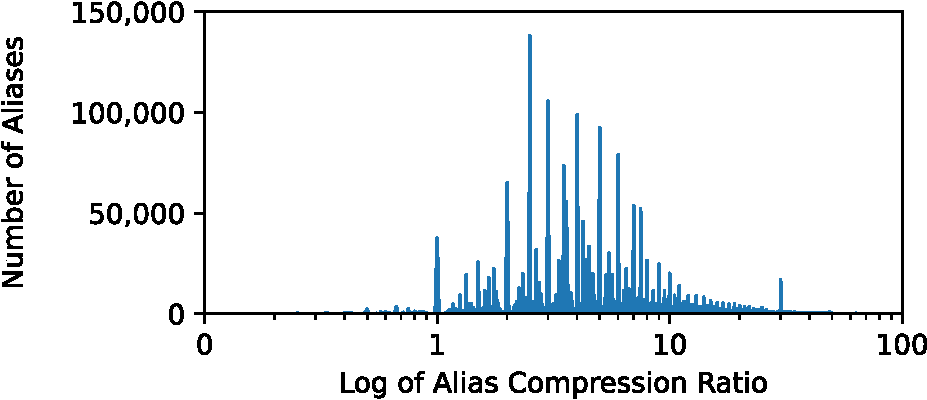
\includegraphics[width=0.95\columnwidth]{figures/compression.pdf}
    \caption{Distribution of alias compression ratios}
    \label{fig:compression}
\end{figure}

\paragraph*{\bf Abbreviating Subcommands}

Many commands can operate in different modes, or act as interfaces to a variety of different \emph{subcommands}.
The subcommand is commonly specified as the first argument to the command, and takes its own set of arguments and flags.
For example, \texttt{git push --tags} executes the \texttt{push} subcommand of \cmd{git} with the \texttt{--tags} flag enabled.
We identified 67 commands in our dataset that take subcommands, such as \cmd{git}, \cmd{docker}, or \cmd{systemctl}.
Noticeably, we found \num{194850} aliases (\per{8.84}) that are purely abbreviations of subcommands, without adding any additional arguments beyond the subcommand.
For example, \alias{gs}{git status} or \alias{gd}{git diff}.
The majority of such subcommand abbreviations (\per{58.5}) are for \cmd{git}, with \num{113980} aliases defined purely for abbreviating \cmd{git} subcommands, accounting for \per{36.77} of all aliases involving \cmd{git}.
The command with the second-most subcommand abbreviations is the package manager \cmd{pacman}, with only \num{9918} instances (\per{5.09} of subcommand abbreviations, but \per{68.67} of all aliases involving \cmd{pacman}).

\paragraph*{\bf Bookmarking Locations}

When an aliased command is called with an argument that references some specific local or remote location, like a file path or domain, the alias acts as a bookmark to that location.
For instance, \alias{starwars}{telnet towel.blinkenlights.nl} and \alias{dl}{cd \textasciitilde/Downloads} are both bookmark aliases.

To find such bookmarking uses in our dataset, we searched for arguments that are locations, which we take to be any of the following:
\begin{itemize}
    \item A string containing a forward slash (\verb|/|), indicating a path.
    \item An IPv4 address, matched by the liberal regular expression \verb|[0-9]+.[0-9]+.[0-9]+.[0-9]+|
    \item A string containing one of the known top-level domains\footnote{\url{http://data.iana.org/TLD/tlds-alpha-by-domain.txt}} preceded by a dot (\verb|.|) and followed by a slash (\verb|/|), colon (\verb|:|) or the end of the string.
\end{itemize}
To avoid false positives, we sampled the top 300 search results according to the above criteria and determined some exclusion patterns.
For instance, \texttt{/dev/null} is not a location for our purposes.
Neither is \texttt{origin/master}, and thus \alias{gm}{git merge origin/master} does not count as a bookmark.
We also exclude aliases that are merely referencing unnamed relative directories (e.g., \verb|../..|).

By our definition, \num{321546} aliases (\per{14.59}) are bookmarks.
Of these, \num{59931} are remote bookmarks containing URLs or IP addresses (\per{15.92} of all bookmarks).
Bookmarks are used predominantly for file system navigation, and the \verb|cd| command is featured heavily.
Most other uses seem to be development related, like starting services such as web servers or databases with pre-defined locations, opening frequently edited files, or outputting logs, as in \alias{onoz}{cat /var/log/errors.log}
%, or opening frequently edited files, as in the most common alias for the most common location, which is for editing the shell configuration itself: \alias{zshconfig}{vim \textasciitilde/.zshrc}.
%\Cref{tab:locations} shows the top local and remote locations found in aliases.

% \begin{table}
%     \caption{Top 5 local and remote locations found in aliases}
%     \label{tab:locations}
%     \begin{tabular}{lr}
    \toprule
    Location & \# \\        
    \midrule
    \verb|~/.zshrc|         &   \num{13331} \\
    \verb|~/.bashrc|        &   \num{7319} \\
    \verb|~/.bash_profile|  &   \num{4403} \\
    \verb|~/.vimrc|         &   \num{3612} \\
    \verb|manage.py|        &   \num{2374} \\
    \midrule
    \verb|myip.opendns.com|         &   \num{2670} \\
    \verb|@resolver1.opendns.com|   &   \num{2645} \\
    \verb|8.8.8.8|                  &   \num{706} \\
    \verb|127.0.0.1|                &   \num{643} \\
    \verb|google.com|               &   \num{461} \\
    \bottomrule
\end{tabular}
% \end{table}


\newcommand{\rot}[1]{\makebox[1em][l]{\rotatebox{45}{#1}}}

\newcommand{\full}{$\CIRCLE$}
\newcommand{\half}{$\LEFTcircle$}
\newcommand{\empt}{$\Circle$}

\newcommand{\hist}[1]{\includegraphics[height=1em, trim=1em 1em 1em 1em, clip]{compression/#1.pdf}}

\newcommand*{\pie}[1]{\begin{tikzpicture}[scale=0.15]%
    \draw (0,0) circle (1);
    \fill[fill opacity=1,fill=black] (0,0) -- (90:1) arc (90:90-#1*3.6:1) -- cycle;
    \end{tikzpicture}}

\begin{table*}
    \caption{\TODO}
    \label{tab:practices-by-command}
    \begin{tabular}{llrlllllllllllllccc}
        & & \# & &\rot{Abbreviating Commands} & \rot{Describing Actions} & \rot{Correcting Misspellings} & \rot{Bookmarking Locations} & & \rot{Substituting Commands} & \rot{Overriding Defaults} & \rot{Colorizing Output} & \rot{Elevating Privilege} & & \rot{Building Tools} & \rot{Transforming Data} & \rot{Chaining Subcommands} & & Compression Ratio \\
        \midrule
        \multicolumn{2}{l}{Version Control} \\
            & \texttt{git} & \num{999999} & & \pie{0} & \pie{0} & \pie{0} & \pie{0} & & \pie{0} & \pie{0} & \pie{0} & \pie{0} & & \pie{0} & \pie{0} & \pie{0} & & \hist{git} \\
            & \texttt{hg} & \num{999999} & & \pie{0} & \pie{0} & \pie{0} & \pie{0} & & \pie{0} & \pie{0} & \pie{0} & \pie{0} & & \pie{0} & \pie{0} & \pie{0} & & \hist{hg} \\
        \midrule
        \multicolumn{2}{l}{System Tools} \\
        & \texttt{ls} & \num{999999} & & \pie{0} & \pie{0} & \pie{0} & \pie{0} & & \pie{0} & \pie{0} & \pie{0} & \pie{0} & & \pie{0} & \pie{0} & \pie{0} & & \hist{ls} \\
        & \texttt{cd} & \num{999999} & & \pie{0} & \pie{0} & \pie{0} & \pie{0} & & \pie{0} & \pie{0} & \pie{0} & \pie{0} & & \pie{0} & \pie{0} & \pie{0} & & \hist{cd} \\
        & \texttt{grep}* & \num{999999} & & \pie{0} & \pie{0} & \pie{0} & \pie{0} & & \pie{0} & \pie{0} & \pie{0} & \pie{0} & & \pie{0} & \pie{0} & \pie{0} & & \hist{grep} \\
        & \texttt{echo} & \num{999999} & & \pie{0} & \pie{0} & \pie{0} & \pie{0} & & \pie{0} & \pie{0} & \pie{0} & \pie{0} & & \pie{0} & \pie{0} & \pie{0} & & \hist{echo} \\
        & \texttt{xargs} & \num{999999} & & \pie{0} & \pie{0} & \pie{0} & \pie{0} & & \pie{0} & \pie{0} & \pie{0} & \pie{0} & & \pie{0} & \pie{0} & \pie{0} & & \hist{xargs} \\
        & \texttt{ssh} & \num{999999} & & \pie{0} & \pie{0} & \pie{0} & \pie{0} & & \pie{0} & \pie{0} & \pie{0} & \pie{0} & & \pie{0} & \pie{0} & \pie{0} & & \hist{ssh} \\
        & \texttt{rm} & \num{999999} & & \pie{0} & \pie{0} & \pie{0} & \pie{0} & & \pie{0} & \pie{0} & \pie{0} & \pie{0} & & \pie{0} & \pie{0} & \pie{0} & & \hist{rm} \\
        & \texttt{dir} & \num{999999} & & \pie{0} & \pie{0} & \pie{0} & \pie{0} & & \pie{0} & \pie{0} & \pie{0} & \pie{0} & & \pie{0} & \pie{0} & \pie{0} & & \hist{dir} \\
        & \texttt{cp} & \num{999999} & & \pie{0} & \pie{0} & \pie{0} & \pie{0} & & \pie{0} & \pie{0} & \pie{0} & \pie{0} & & \pie{0} & \pie{0} & \pie{0} & & \hist{cp} \\
        & \texttt{mv} & \num{999999} & & \pie{0} & \pie{0} & \pie{0} & \pie{0} & & \pie{0} & \pie{0} & \pie{0} & \pie{0} & & \pie{0} & \pie{0} & \pie{0} & & \hist{mv} \\
        & \texttt{sort} & \num{999999} & & \pie{0} & \pie{0} & \pie{0} & \pie{0} & & \pie{0} & \pie{0} & \pie{0} & \pie{0} & & \pie{0} & \pie{0} & \pie{0} & & \hist{sort} \\
        & \texttt{head} & \num{999999} & & \pie{0} & \pie{0} & \pie{0} & \pie{0} & & \pie{0} & \pie{0} & \pie{0} & \pie{0} & & \pie{0} & \pie{0} & \pie{0} & & \hist{head} \\
        & \texttt{cat} & \num{999999} & & \pie{0} & \pie{0} & \pie{0} & \pie{0} & & \pie{0} & \pie{0} & \pie{0} & \pie{0} & & \pie{0} & \pie{0} & \pie{0} & & \hist{cat} \\
        \midrule
        \multicolumn{2}{l}{Package Managers} \\
        & \texttt{apt}* & \num{999999} & & \pie{0} & \pie{0} & \pie{0} & \pie{0} & & \pie{0} & \pie{0} & \pie{0} & \pie{0} & & \pie{0} & \pie{0} & \pie{0} & & \hist{apt} \\
        & \texttt{zypper} & \num{999999} & & \pie{0} & \pie{0} & \pie{0} & \pie{0} & & \pie{0} & \pie{0} & \pie{0} & \pie{0} & & \pie{0} & \pie{0} & \pie{0} & & \hist{zypper} \\
        & \texttt{pacman} & \num{999999} & & \pie{0} & \pie{0} & \pie{0} & \pie{0} & & \pie{0} & \pie{0} & \pie{0} & \pie{0} & & \pie{0} & \pie{0} & \pie{0} & & \hist{pacman} \\
        & \texttt{mvn} & \num{999999} & & \pie{0} & \pie{0} & \pie{0} & \pie{0} & & \pie{0} & \pie{0} & \pie{0} & \pie{0} & & \pie{0} & \pie{0} & \pie{0} & & \hist{mvn} \\
        & \texttt{yaourt} & \num{999999} & & \pie{0} & \pie{0} & \pie{0} & \pie{0} & & \pie{0} & \pie{0} & \pie{0} & \pie{0} & & \pie{0} & \pie{0} & \pie{0} & & \hist{yaourt} \\
        & \texttt{brew} & \num{999999} & & \pie{0} & \pie{0} & \pie{0} & \pie{0} & & \pie{0} & \pie{0} & \pie{0} & \pie{0} & & \pie{0} & \pie{0} & \pie{0} & & \hist{brew} \\
        & \texttt{port} & \num{999999} & & \pie{0} & \pie{0} & \pie{0} & \pie{0} & & \pie{0} & \pie{0} & \pie{0} & \pie{0} & & \pie{0} & \pie{0} & \pie{0} & & \hist{port} \\
        \midrule
        \multicolumn{2}{l}{Text Editors}  \\
        & \texttt{mate} & \num{999999} & & \pie{0} & \pie{0} & \pie{0} & \pie{0} & & \pie{0} & \pie{0} & \pie{0} & \pie{0} & & \pie{0} & \pie{0} & \pie{0} & & \hist{mate} \\
        & \texttt{vim} & \num{999999} & & \pie{0} & \pie{0} & \pie{0} & \pie{0} & & \pie{0} & \pie{0} & \pie{0} & \pie{0} & & \pie{0} & \pie{0} & \pie{0} & & \hist{vim} \\
        & \texttt{nvim} & \num{999999} & & \pie{0} & \pie{0} & \pie{0} & \pie{0} & & \pie{0} & \pie{0} & \pie{0} & \pie{0} & & \pie{0} & \pie{0} & \pie{0} & & \hist{nvim} \\
        & \texttt{emacs} & \num{999999} & & \pie{0} & \pie{0} & \pie{0} & \pie{0} & & \pie{0} & \pie{0} & \pie{0} & \pie{0} & & \pie{0} & \pie{0} & \pie{0} & & \hist{emacs} \\
        \midrule
        \multicolumn{2}{l}{Infrastructure} \\
        & \texttt{docker}* & \num{999999} & & \pie{0} & \pie{0} & \pie{0} & \pie{0} & & \pie{0} & \pie{0} & \pie{0} & \pie{0} & & \pie{0} & \pie{0} & \pie{0} & & \hist{docker} \\
        & \texttt{kubectl}* & \num{999999} & & \pie{0} & \pie{0} & \pie{0} & \pie{0} & & \pie{0} & \pie{0} & \pie{0} & \pie{0} & & \pie{0} & \pie{0} & \pie{0} & & \hist{kubectl} \\
        & \texttt{vagrant} & \num{999999} & & \pie{0} & \pie{0} & \pie{0} & \pie{0} & & \pie{0} & \pie{0} & \pie{0} & \pie{0} & & \pie{0} & \pie{0} & \pie{0} & & \hist{vagrant} \\
        \midrule
        \multicolumn{2}{l}{Other} \\
        & \texttt{ffmpeg} & \num{999999} & & \pie{0} & \pie{0} & \pie{0} & \pie{0} & & \pie{0} & \pie{0} & \pie{0} & \pie{0} & & \pie{0} & \pie{0} & \pie{0} & & \hist{ffmpeg} \\
        & \texttt{beep} & \num{999999} & & \pie{0} & \pie{0} & \pie{0} & \pie{0} & & \pie{0} & \pie{0} & \pie{0} & \pie{0} & & \pie{0} & \pie{0} & \pie{0} & & \hist{beep} \\
    \end{tabular}
\end{table*}


\subsection{Modifications}

Aliases are not only used syntactically, for naming purposes, but also in ways that change the semantics of certain commands.
We found four customization practices related to command modification.

\paragraph*{\bf Substituting Commands}

When an alias name is identical to the name of a pre-existing command, the alias defines a substitution for that command.
A common example is \alias{more}{less}, replacing a standard Unix utility (\cmd{more}) with a more capable but similar command (\cmd{less}).
This can also be used for subterfuge, as in \alias{emacs}{vim} (appearing 132 times in our dataset) or indeed \alias{vim}{emacs} (86 times, alas).

To determine which alias names are also actual command names, we compared them to known Unix commands\footnote{\url{https://en.wikipedia.org/wiki/List_of_Unix_commands}\\ and \url{https://en.wikipedia.org/wiki/List_of_GNU_Core_Utilities_commands}} and a curated sample of commands from our dataset (taking care to not include names that appear in a command position but are actually just other aliases).
To determine proper substitutions, we only count aliases whose value does not also include the name of the command (which would point to an overriding alias, see below).
We find that \num{100564} aliases (\per{4.56}) are used to substitute one command for another.
The top three substitutions are \verb|vi| $\rightarrow$ \verb|vim|, \verb|vim| $\rightarrow$ \verb|nvim|, and \verb|vi| $\rightarrow$ \verb|nvim|.

\paragraph*{\bf Overriding Defaults}

When an alias has the same name as the command it aliases, as in \alias{ls}{ls -G}, then the alias re-defines the command and effectively overrides its default settings.
Any time the command is now executed, it will be with the arguments specified in the alias.
There are \num{319239} aliases in our dataset (\per{14.48}) that are used to override defaults in this way.
Aliases to override the defaults of the \cmd{grep} family of commands (\cmd{grep}, \cmd{egrep}, \cmd{fgrep}) occur \num{96970} times, accounting for \per{4.4} of all alias definitions (and \per{68.27} of all \cmd{grep} appearances).
The \cmd{ls} command is redefined with new defaults \num{75374} times, accounting for \per{3.42} of all aliases (\per{28.99} of \cmd{ls} appearances).

Looking at the new defaults of these redefined commands, they reveal a variety of user preferences, especially in the diverse long tail, where we find a lot of unique alias definitions and argument combinations.
Two areas of customization stand out, however: formatting output and adding safety.
The majority of overrides for file system commands (\cmd{mv}, \cmd{cp}, and \cmd{rm}, but also \cmd{ln}, for creating symbolic links) enable interactive mode (\texttt{-i} and variations), which prompts the user before performing potentially destructive actions.
Verbose output (\texttt{-v}) also plays a role here, describing exactly what kind of effects a command execution had or will have.
Enabling verbosity can also be seen as a kind of output formatting, although much more common is the wish for human-readable output.
For example, the alias \alias{df}{df -h} ensures that the available disk space is displayed in common size units, as opposed to just the raw number of bytes.
But by far the most common reason for overriding defaults is to enable colorized output.
This behavior is so prevalent that we count it as a customization practice in its own right.

\paragraph*{\bf Colorizing Output}

Enabling colored output can be done in many different ways: adding an argument (like \texttt{less -R} or \cmd{grep --color=always}), setting an environment variable (as in \alias{ssh}{TERM=xterm256color ssh}), running the command through a tool that colorizes its output (like \cmd{grcat} or \cmd{pygmentize}), or even replacing a command outright (\alias{diff}{colordiff}).
Taking all these varieties into account, more than half of all command redefinitions (\per{57.21}) enable colored output by default.
This amounts to a surprising \num{182623} aliases, or \per{8.29} percent of all aliases in the dataset.
If we extend this count to also include aliases that introduce new names (like \alias{ll}{ls -l --color=auto}), then more than \per{10} of aliases colorize a command's output.

\paragraph*{\bf Elevating Privilege}

The \cmd{sudo} command allows the user to execute another command with superuser privileges.
Combining a command with \cmd{sudo} is often necessary if the other command needs to modify critical parts of the system.
In our dataset, we found \num{93683} aliases (\per{4.25}) in which a command is prefixed with \cmd{sudo}.
The top \cmd{sudo}-prefixed command is the package manager \cmd{apt-get}, appearing \num{10467} times with \cmd{sudo}.
Remarkably, these are \per{89.35} of all occurrences of \cmd{apt-get}.
In fact, \per{72.45} of all occurrences of the package managers \cmd{apt}* (Debian and derivatives; including \cmd{apt}, \cmd{apt-get}, \cmd{apt-cache}, \cmd{aptitude}, and \cmd{\$apt\_pref}), \cmd{pacman}, \cmd{abs} and \cmd{aur} (Arch Linux), \cmd{yum} (RPM), \cmd{dnf} (Fedora), \cmd{zypper} (openSUSE), \cmd{port} (macOS), and \cmd{gem} (Ruby) are together with \cmd{sudo}, and these package managers account for \per{29.1} of all \cmd{sudo} occurrences.
Interestingly, the macOS package manager \cmd{brew} rarely appears with \cmd{sudo} (only \per{1.07}), even though it is the third most occurring package manager overall, behind \cmd{apt}* and \cmd{pacman}.

Other commands that more often than not demand elevated privileges are system utilities like \cmd{systemctl}, \cmd{shutdown}, \cmd{lsof} or \cmd{mount}.

\subsection{Scripts}

Aliases that combine multiple commands are basically tiny shell scripts.
In our dataset, \num{204142} aliases (\per{9.26}) compose multiple commands.
The most popular composition operator is the pipe (\verb`|`), used in \per{39.66} percent of alias scripts, followed by the operators for simple chaining (\verb|;|), with \per{29.61}, and logical conjunction (\verb|&&|), with \per{26.88}.
Other operators (\verb`||`, \verb`|&`) appear in only \per{3.85} of multi-command aliases.

There are two scripting practices that are of particular interest.

\paragraph*{\bf Transforming Data}

The pipe (\verb`|`) creates an interface between two otherwise separate programs.
It embodies the Unix philosophy of small tools doing one thing well, which can then be connected together to accomplish more complex tasks.
There are \num{74719} aliases (\per{3.39}) combining two or more commands using only the pipe operator.
The most common command occurring after a pipe, by far, is \cmd{grep}, which makes an appearance in almost half of all pipelines (\per{46.16}), more than three times as often as \cmd{xargs} and \cmd{sort}.
The most common data sources are \cmd{ps}, \cmd{git}, and \cmd{ls}, which are found at the beginning of almost a third (\per{32}) of all pipelines.
\Cref{fig:flow} shows a flow diagram of the top pipelines with three commands.

\begin{figure*}[h]
	\centering    
	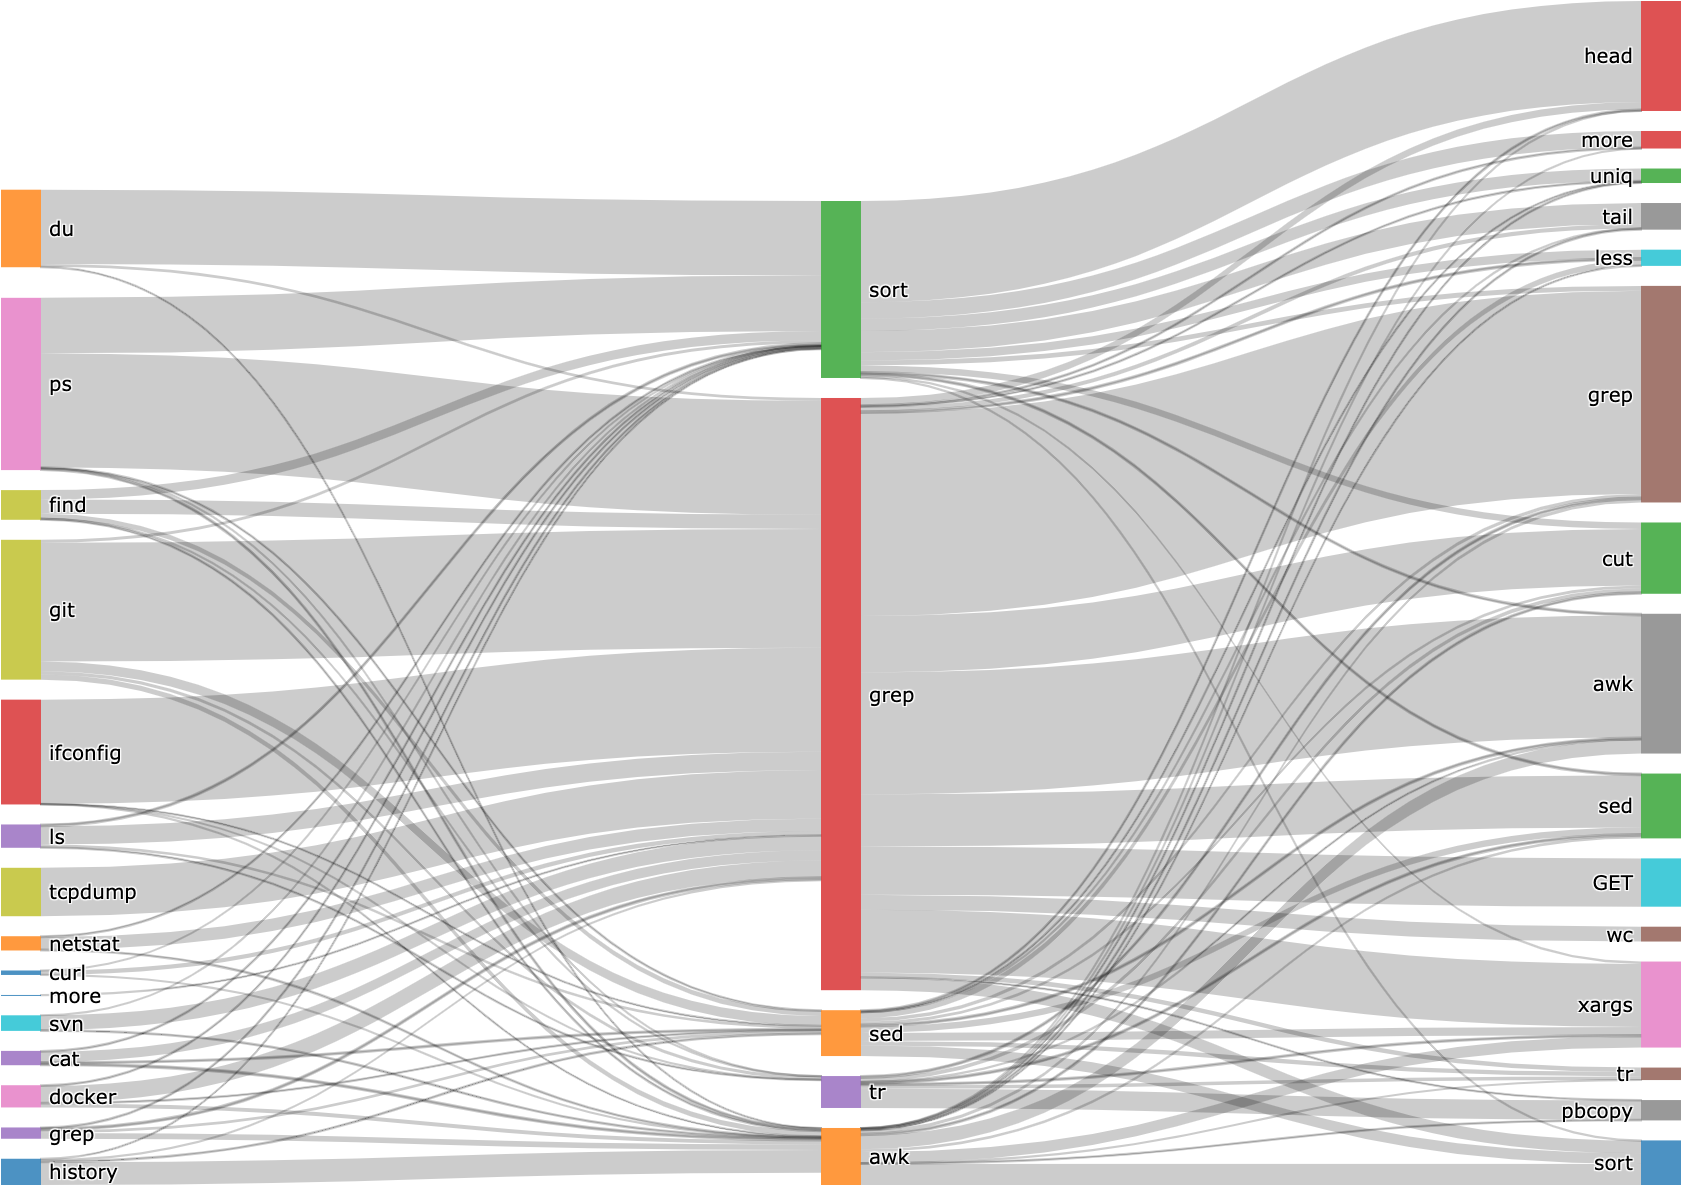
\includegraphics[width=0.78\linewidth]{figures/flow_250.png}
	\caption{Flow diagram of the top 250 pipelines with three commands that make up at least \per{10} of one participating command's usage}
	\label{fig:flow}
\end{figure*}

\paragraph*{\bf Chaining Subcommands}

An interesting pattern appearing in alias scripts are chains of subcommand invocations.
For example, the package manager \cmd{brew} has a subcommand \texttt{update}, for updating the package database, and a subcommand \texttt{upgrade}, for upgrading previously installed packages to the latest available versions.
\per{28.08} percent of all aliases involving the \cmd{brew} command contain the composition \verb|brew update && brew upgrade| (sometimes with \verb|;| instead of \verb|&&|), with alias names like \verb|update|, \verb|brewup|, \verb|bup|, etc.
This pattern of repeated subcommand invocations can be found in \num{22062} aliases (\per{1}), and it is most prevalent among package managers, like \cmd{brew}, \cmd{apt-get}, \cmd{npm} or \cmd{gem}, mostly for the same purpose as in the \cmd{brew} example.

The command with the highest absolute number of aliases showing this pattern is \cmd{git}, however, with \num{12063} occurrences (\per{3.89} of all aliases using \cmd{git}).
Here, the uses are more varied, 
e.g., \alias{commit}{git add . \&\& git commit -m}, 
or \alias{gitpull}{git stash \&\& git pull \&\& git stash pop},
or indeed \alias{whoops}{git reset --hard \&\& git clean -df}.


\section{Implications}

Through our large-scale analysis 
%of unique files that contain over 2.2 million alias definitions, 
we gained insight into practices detailing how users customize their command-line interface.
Based on our observations, we outline discussion points that go beyond single customization practices and identify implications that can address shortcomings in command-line usability and tie them to existing user experience research.
Further, while our presented findings already give us an understanding of customization practices over many different kinds of commands, we view our collected dataset as a playground for fine-grained discovery that can benefit researchers, tool builders, and command-line users.

\paragraph{Learning Repair Rules}

The complexity of commands and arguments can cause users to introduce errors when working in a command line interface.
Figuring out specifically how to fix these errors is often a convoluted process.
A popular open source project that attempts to navigate this issue\footnote{\url{https://github.com/nvbn/thefuck}} uses a set of rules to suggest possible error corrections for commands.
While these rules are all hard-coded, we envision leveraging the global wisdom of customizations in our large-scale dataset to learn rules that form the basis for different kinds of suggestions.
This is in line with work in leveraging emergent behavior from corpora~\citep{fast:14} that we can codify based on our customization data.
%An obvious choice from our analysis are autocorrecting aliases to learn repair rules.

\paragraph{Discovering Workflows}
Following a different thread of leveraging emergent practices, we can also see how our dataset would enable a world beyond only trying to fix immediate errors, by providing usage hints that could introduce users to common parameters and workflows.
For example, as soon as a user tries to \cmd{sort} the output of the \cmd{ps} command, the alias \alias{mem10}{ps auxf | sort -nr -k 4 | head -10} can serve as a suggestion for the complex but common data transformation that results in showing the ten most memory-intensive processes.
%\paragraph*{\bf Object Protocols}
Similarly, in the practice of \emph{chaining subcommands} we can clearly see the prevalence of object protocols~\citep{beckman:11}, which are implicit rules determining the order in which commands have to be executed.
We can improve usability by enabling the discovery of these implicit rules and by exposing the dependency structure based on our customization data.
For instance, if executing \verb|brew upgrade| results in a failure, we can suggest using \verb|brew update && brew upgrade| instead, based on the patterns in our dataset. 

\paragraph{Uncovering Conceptual Design Flaws}

Customization can also be an indicator for problems in the underlying conceptual design, manifesting as usability frustrations that require adaptation by the user.
Briefly comparing our findings to the qualitative analysis on conceptual design flaws in \cmd{git} by \cite{perez:13}, we can clearly see the same frustrations with committing and switching branches,\footnote{``Just Let Me Commit!" and ``I Just Want to Switch Branches" in \cite{perez:13}} based on the alias definitions in our dataset (e.g., \alias{commit}{git add . \&\& git commit -m}).

We want to emphasize that we are not suggesting that large-scale quantitative data of customization practices can replace qualitative analysis, but rather that the corpus we provide, together with our findings, can support exploration and provide new insights for usability research.

\paragraph{Contextual Defaults}

Choosing proper defaults in user interfaces is a pillar of user experience design~\citep{nielsen2005power}.
The fact that \per{14.48} of the customizations in our dataset are for \emph{overriding defaults} suggests that, at least for some groups of users, the default settings of their tools could be improved.
We see \emph{overriding defaults} not necessarily as an indictment of the involved commands, but rather as an indication that the assumed user context does not in all cases match the actual usage profile.
Indeed, the variety of different defaults in the data indicate what we call \emph{contextual} defaults, where context could be a reflection of the level of expertise of a command-line user, or a certain persona (e.g., system administrator, data scientist, or software engineer).
We could imagine providing different sets of defaults to different users, effectively alias starter packs, generated from our data.
We see parallels to work that investigates contextual preferences and personalization in information systems~\citep{de:15, stefanidis:11} and privacy research~\citep{wijesekera:18, alom:19}. 

\paragraph{Interactivity vs Batch-Processing}

Context extends to the environment a command is executed in, particularly whether it is used on an interactive command-line or as part of a script for batch-processing.
Our findings highlight the tension between these different ways of execution and how a human user can have needs different from an automated workflow.
This particularly comes to light in the customization practices of \emph{colorizing output} and \emph{overriding defaults}.
While human-readable output or prompting for destructive actions makes no sense in scripts and is usually seen as cumbersome for expert users even on the command-line, our findings show that aliases like \alias{mv}{mv -i} are nonetheless highly desired by some.


\section{Threats to Validity}

We review potential limitations of our study as threats to validity.
First, our sample might not be representative.
Our dataset only includes aliases by people who publicly shared their dotfiles, we only collected from GitHub, and our sample does not include forks.
Nevertheless, our dataset is very exhaustive, as we were able to sample \per{94.09} of the estimated population of Shell files containing aliases on GitHub.
And while mining GitHub can be fraught with perils \citep{kalliamvakou:14}, we specifically sought out personal repositories, side-stepping many of the typical issues with mining GitHub for software projects.

Second, our parser might not be sophisticated enough to recognize complex real-world aliases or cope with minute platform differences.
To mitigate this threat, we ran multiple sanity checks and tested the parser on some hairy examples from the dataset.
We did not detect any significant mis-parses and think that we have covered the majority of relevant cases.
The raw unparsed database is available in our replication package.

Third, aliases might not reflect intent as much as we assume.
En-masse copy-pasting of aliases by users, without them knowing exactly what they are copying, is certainly a realistic scenario.
System distributions and configuration frameworks like \emph{ohmyzsh} ship with numerous aliases by default or as part of easily enabled plugins.
Users might not even be aware of the aliases they have on their system.
We mitigate this concern by removing all duplicate files from our dataset that would indicate sheer copy/pasting.
%We also particularly exclude alias definitions that come bundled with operating systems and particular shells (e.g., zsh).
%This is mitigated by the fact that all of the aliases we collected were publicly shared by users.
%It stands to reason that even if a user is not aware of all the details of their system configuration, they confirm their attachment to this configuration and its aliases by publicly sharing them---even if only for the purposes of synchronizing them across the users' own machines.

Fourth, we might not actually be able to see the true user intent, if it exists, as quantitative measures might hide a long tail of minor variations and individual user preference.
Conclusions about common aliases or selected subsets might not be generalizable.
To mitigate these summarizing effects, we established customization practices as a vehicle to take a deeper dive into the details of certain alias usage.
Since we sampled almost the whole available population, we are confident in the strength of our data and the conclusions we can draw from particular instances.
Our replication package includes our whole toolchain and all alias data in a relational format ready for further analysis.


\section{Related Work}

Related research in the broader context of our work has been conducted on the use of command-line interfaces and how to improve it, and the shell as a programming language for both scripting and interactive use. 

The earliest related study we found was by \cite{greenberg:88a}, which collected four months of continuous real-life use of the Unix \verb|csh| shell from 168 users. 
The data was used in a follow up study to analyze the use of interactive systems by examining frequency of command invocations for different groups of users~\citep{greenberg:88b}.
In later work, \cite{davison:98} use probabilistic action modeling to predict user action sequences based on the same dataset.
\cite{korvemaker:00} similarly predict future action sequences in command lines, but condition on actions of the particular user group with the goal of enabling adaptive user interfaces.
Other work in the context of adaptive user interfaces by \cite{jacobs:01} uses association rule learning on the shell logs to produce scripts to automate common task sequences.
\cite{khosmood:14} use the same corpus and two additional, more recent, corpora to learn a model that can identify user profiles based on their command-line behavior.
Bespoke~\citep{bespoke:19} is a system that synthesizes specialized graphical user interfaces (GUIs) based on command usage.
Our work can be viewed as an input to this system that passes common shell workflows in aliases to be generated as GUIs.

There has been other work on enhancing user experience in command-line interfaces.
NoFAQ~\citep{dantoni:17} provides repair suggestions for failed shell invocations based on a model learned from a curated set of fix patterns.
NL2Bash~\citep{lin:18} implements a system that translates natural language phrases in English to shell commands.
Recent work by \cite{greenberg:17} has been looking into understanding the POSIX shell as a programming language.
More specifically, understanding word expansion in the shell to support interactivity~\citep{greenberg:18a} and concurrency~\citep{greenberg:18b}.


\section{Conclusion}

We report on a large scale exploratory study on how command line users customize user experience by defining shell aliases.
Through inductive coding, 9 customization practices emerged from our dataset that provide insight on the characteristics of command-line use.
Based on our results, we discuss and formulate a set of implications for command-line tool developers, researchers, and the shell as an interactive environment for experts.

Aliases often redefine commands with other default arguments, which is a potential indicator for usability problems in these tools.
However, we have to also be aware that defaults can be highly contextual depending on user profiles (e.g., expertise level) and environment (e.g., scripting vs. interactive use).
We also see our dataset and results as a rich source for learning norms with respect to repair rules, data flows, and descriptive names for complex command structures.
We provide a comprehensive replication package and see potential for future work based on our dataset and analyses.

\bibliographystyle{spbasic}
\bibliography{references}

\end{document}
